\section{Introduction}

This document will serve as a comprehensive guide through the entire power distribution and wiring system of our rover. It meticulously details all relevant safety measures designed to minimize the likelihood of hazards or environmental damage. By following these guidelines, we aim to ensure that our work adheres to the highest safety standards.\\

In addition to outlining essential safety protocols, this guide sets forth the minimum standards for both material and personal safety. These standards apply not only during the construction phase but also throughout the actual operation of all electronic components. To enhance understanding and clarity, we have included several schematics, data sheets, and detailed calculations. These resources are designed to provide a thorough illustration of the rover's internal architecture and functionality, making the document as informative and accessible as possible.

\section{Hazardous Material List}

Dino-bot's power architecture consists of an energy storage module, an emergency stop system, a main
power distribution system, a secondary power distribution and several
downstream devices.


The legend for the rover systems architecture, and the detailed circuit diagrams is
shown below.
The rover uses 5 standard voltages for the distribution. These are unregulated 22.2v
from the battery, a regulated 12v for linear actuators and Arduino Mega, a regulated 9v
four ip cameras, a regulated 6.5v for servo motors and regulated 5v for Rasperry Pi’s.

\newpage



\newpage
\section{Power Architecture}

The rover's power architecture is divided into two separate power systems. This approach ensures galvanic isolation between the power and logic components, which is necessary to eliminate any possible wiring configuration in which a so-called "ground loop" could form. The underlying problem is based on the fact that there exists an interface and thus an electrical connection between the individual components. While the communication between power and logic components is implemented by establishing a physical connection between their corresponding GPIO pins and reading different voltage levels, there must be a precise reference voltage available. Generally speaking, this is done by using a common ground. Hence, the most basic form to utilize that common ground connection is to form a "star ground." If there are multiple paths to ground, a "ground loop" is present. These ground loops, in combination with wire inductance, can cause issues for high-current electronics like our motor controller (electronic speed controller). This is further illustrated in Figure XY.

\begin{figure}[h]
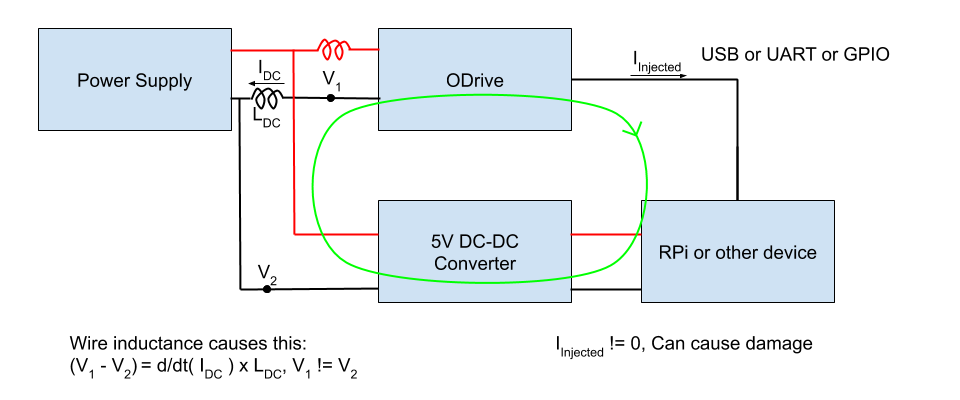
\includegraphics[width=\textwidth]{contents/figures/ground_loop_bad.png}
\end{figure}




\section{Energy Storage}

\section{Emergency Stop}

\section{Power Distribution}

\section{Power Conversion}

\section{Power Consuming Circuits}

\section{Unused Circuits}

\section{Circuit Table}




